
\section*{Ejercicios}
\addcontentsline{toc}{section}{\textit{Ejercicios}}
\begin{Enunciado}
\subsection*{Ejercicio 1}

Cuestiones sobre la resistividad y movilidad:
\begin{enumerate}[label=\alph*)]
	\item La resistividad de un material tipo N es por lo regular más pequeña que la resistividad de un material tipo P de dopado comparable, explica por qué suele ocurrir esto. Calcula la resistividad del Si si se dopa con fósforo con una concentración de \( 10^{17} \) cm\(^{-3}\). Repite el cálculo para el caso en que dopemos con aluminio con la misma concentración y calcular la corriente de arrastre en ambos casos considerando un campo eléctrico de \( 10^5 \) V/cm.

	\item Calcula la densidad de impurezas necesarias para tener un cristal de Si tipo P con resistividad 0.1 \(\Omega\cdot\)cm. ¿Qué proporción hay de átomos de impureza sobre el número de átomos de Si?
		  (DATO: Constante de red del Si \( a_0 = 5.431 \) Å). Si suponemos que el semiconductor es no degenerado, ¿cuánto vale \( D_p \)?
\end{enumerate}

\end{Enunciado}




\begin{enumerate}[label=\alph*)]
	\item La diferentencia radica en la masa efectiva, que se expresa en la movilidad:
		  \begin{equation}
			  \rho = \frac{1}{q(n\mu_n + p \mu_)}
		  \end{equation}
		  Cuando $\mu_n>\mu_p \Rightarrow \rho_n < \rho_p$. Y esto siempre ocurre. Las movilidades dependen de la temperatura y la cantidad que esté dopado, por lo que puede ser diferente. Para un semiconductor dopado tipo $N$:

		  \begin{equation}
			  \rho_N = \frac{1}{qn{\mu_n}} = \frac{1}{1.6\cdot 10^{19} \cdot 10^{17}\cdot 1350}= 0.0463 \Omega \cm
		  \end{equation}
		  Y para un tipo $P$:
		  \begin{equation}
			  \rho_N = \frac{1}{1.6\cdot 10^{19} \cdot 10^{17}\cdot 480} = 0.13 \Omega \cm
		  \end{equation}
		  (valores de movilidad sacados de la Wikipedia). Ahora podemos calucular la corriente de arrastre (usamos que $J=qnN\epsilon$, donde $\epsilon = 10^5$ eV)
		  \begin{equation}
			  J_N =  2.16 \cdot 10^6  A\cm^{-2}  \tquad J_p = 7.68 \cdot 10^3  A\cm^{-2}
		  \end{equation}
	\item Ahora lo que hacemos es considerar que el número de impurezas es igual al número de huecos (están todas completamente ionizadas). Lo que nos queda entonces es:
		  \begin{equation}
			  N_A = \frac{1}{q\rho \mu_p } = \frac{1}{1.6\cdot 10^{19} \cdot 0.1 \cdot 480} = 1.3 \cdot 10^{17} \cm^{-3}
		  \end{equation}
		  Podemos calcular con $a_0$ el númerode átomos de silicio por unidad de volumen:

		  \begin{equation}
			  N_{Si} = 5 \cdot 10^{22} \text{at} \cm^{-3}
		  \end{equation}
		  Y solo tenemos, para calcular la proporción:

		  \begin{equation}
			  \frac{N_A}{N_{Si}} = 2.6 \cdot 10^{-6} = 2.6 \ \text{ppm}
		  \end{equation}
		  Para acabar necesitamos calcular la relación de Eistein (solo usable en semicdonductores no degenerados). Así tenemos que

		  \begin{equation}
			  D_p = \frac{kT}{q} \mu_p = 12.4 \cm^2 / s
		  \end{equation}
\end{enumerate}

\begin{Enunciado}
\subsection*{Ejercicio 2}

Responde a las siguientes cuestiones:
\begin{enumerate}
	\item[a)] Calcular la resistividad del GaAs intrínseco a temperatura ambiente ($\mu_n = 9200$ cm$^2$/Vs, $\mu_p = 320$ cm$^2$/Vs).

	\item[b)] La movilidad de los electrones en el silicio es $\mu_n = 1300$ cm$^2$/Vs a temperatura ambiente. Si asumimos que la movilidad está limitada principalmente por la dispersión con la red cristalina, calcular la movilidad a $T= 150$ K.

	\item[c)] Dos mecanismos de dispersión tienen lugar en un semiconductor. Si sólo el primer de los mecanismos está presente la movilidad es de 250 cm$^2$/Vs. Si sólo el segundo de los mecanismos está presente la movilidad es de 650 cm$^2$/Vs. Calcular la movilidad cuando los dos mecanismos están presentes.
\end{enumerate}

\end{Enunciado}



\begin{enumerate}[label=\alph*)]
	\item Para calcular la resistividad usamos la fórmula:
	\begin{equation}
		\rho = \frac{1}{q(\mu_p p + \mu_n n )}
	\end{equation}
	Donde solo tenemos que sustituir $n,p\rightarrow n_i$. Calculamos usando que $n_i= 2.25\times 10^6 \cm^{-3}$ de lo que se deduce que:
	\begin{equation}
	\rho =4.33\cdot 10^9 \ \Omega \cm
	\end{equation}
	\textcolor{Blue}{Creo que hay algo mal en el resultado numérico aunque la ecuación está bien. Podría dar entorno a 2.5 por diez a la diez, más o menos.}
	\item No conocemos la fórmula explícita, pero śi que sabemos que $\mu_{\text{impurezas}}\propto T^{-3/2}$ (red cristalina es igual a dispersión por fonones). Por tanto podemos calcular:
	\begin{equation}
		\frac{\mu_{\text{imp}} (T=150K)}{\mu_{\text{imp}}(T=300K)} = \parentesis{\frac{150}{300}}^{-3/2}		
	\end{equation}
	De lo que obtenemos:
	\begin{equation}
		\mu_{\text{imp}} (T=150K) = 3677 \ \cm^2 / \text{Vs}
	\end{equation}
	\item Tenemos que usar la \textit{regla mathiessen}:
	\begin{equation}
		\frac{1}{\mu} = \frac{1}{\mu_{1}}+\frac{1}{\mu_{2}} 
	\end{equation}
	De lo que obtenemos:		
	\begin{equation}
		\mu = 180.55 \ \cm^2 / \text{Vs} 
	\end{equation}
\end{enumerate}

\begin{Enunciado}
\subsection*{Ejercicio 3}
Obtener las concentraciones de electrones y huecos, movilidades y resistividades de muestras de silicio a \(300 K\) para las siguientes concentraciones de impurezas:
\begin{itemize}
	\item[(a)] \(1 \times 10^{15}\) átomos/cm$^3$ de boro.
	\item[(b)] \(1 \times 10^{16}\) átomos/cm$^3$ de boro y \(1.5 \times 10^{16}\) átomos/cm$^3$ de arsénico.
	\item[(c)] \(5 \times 10^{15}\) átomos/cm$^3$ de boro, \(10^{17}\) átomos/cm$^3$ de arsénico y \(10^{17}\) átomos/cm$^3$ de galio.
\end{itemize}
Considerar que, las movilidades para portadores mayoritarios:
\begin{equation}
	\mu_n (N) = 65  + \frac{1265}{1+\parentesis{\frac{N}{8.5\times 10^{16}}}^{0.72}} \qquad 
	\mu_p (N) = 48  + \frac{447}{1+\parentesis{\frac{N}{6.3\times 10^{16}}}^{0.76}}
\end{equation}
Para portadores minoritarios:
\begin{equation}
	\mu_n (N) = 232  + \frac{1180}{1+\parentesis{\frac{N}{8\times 10^{16}}}^{0.9}} \qquad 
	\mu_p (N) = 130  + \frac{370}{1+\parentesis{\frac{N}{8\times 10^{17}}}^{1.25}}
\end{equation}

\end{Enunciado}




Primero tenemos que evaluar si son dadores/aceptores, calcular $n$ y $p$, luego evaluar las fórmulas para portadores mayoritarios y minoritarios, y finalmente la resistividad. \textcolor{red}{Tengo que cambiar los datos, ya que $N=N_A+N_D$, teniendo que calcular n y p de una manera difernte a $p=N_D$.}  Para calcular $n$ y $p$:
\begin{enumerate}[label=\alph*)]
	\item El Boro es un átomo aceptor, por lo que tendremos como dato $N_A=10^{15} \ $átomos/$\cm^3$. Ahora calculamos, usando que $n_i=1.18\times 10^{10}$:   
	\begin{equation}
		p = N_A = 10^{15} \qquad n = \frac{n_i^2}{p} =1.39 \cdot 10^5 \cm^-3
	\end{equation}
	Calculamos las movilidades, usando la mayoritaria para los huecos y la minoritaria para los electrones:
	\begin{equation}
		\mu_p=4.77\cdot 10^2  \ \cm^2 /  \text{V s} \qquad 
		\mu_n=1.39 \cdot 10^3 \ \cm^2 /  \text{V s}
	\end{equation}
	La resistividad $\rho$ se calcula ahora fácilmente:
	\begin{equation}
		\rho = \frac{1}{e(\mu_n n + \mu_pp)} \rightarrow 
		\rho = 13.1 \ \Omega \cm
	\end{equation}

	\item El Arsénico es un átomo dador, por lo que tendremos como dato $N_{D\text{eff}}=5 \times 10^{15} \ $átomos/$\cm^3$, que se deduce de:
	\begin{equation}
		N_{D\text{eff}} = N_{\text{As}} - N_{\text{B}} = 5 \times 10^{15}
	\end{equation}
	Ahora calculamos, usando que $n_i=1.18\times 10^{10}$:   
	\begin{equation}
		n = N_{D\text{eff}} = 10^{15} \qquad p = \frac{n_i^2}{n} = 2.78 \cdot 10^4 \cm^-3
	\end{equation}
	Calculamos las movilidades, usando la mayoritaria para los electrones y la minoritaria para los huecos:
	\begin{equation}
		\mu_n=9.60 \cdot 10^2  \ \cm^2 /  \text{V s} \qquad 
		\mu_p=4.89 \cdot 10^2  \ \cm^2 /  \text{V s}
	\end{equation}
	La resistividad $\rho$ se calcula ahora fácilmente:
	\begin{equation}
		\rho = \frac{1}{e(\mu_n n + \mu_pp)} \rightarrow \rho = 1.3 \ \Omega \cm
	\end{equation}
	ESTA TODO MAL.
	\item El Galio es un átomo aceptor, por lo que tendremos como dato $N_{A\text{eff}}=5 \times 10^{15} \ $átomos/$\cm^3$, que se deduce de:
	\begin{equation}
		N_{A\text{eff}} = N_{\text{Ga}} + N_{\text{B}} - N_{\text{As}} =  2.78 \cdot 10^4 \ \cm^{-3}
	\end{equation}
	Ahora calculamos, usando que $n_i=1.18\times 10^{10}$:   
	\begin{equation}
		p = N_{A\text{eff}} = 5 \times 10^{15} \qquad p = \frac{n_i^2}{n} = 3e+04 \cm^-3
	\end{equation}
	Calculamos las movilidades, usando la mayoritaria para los huecos y la minoritaria para los electrones:
	\begin{equation}
		\mu_p=4.38 \cdot 10^{2}  \ \cm^2 /  \text{V s} \qquad 
		\mu_n=1.18 \cdot 10^{3} \ \cm^2 /  \text{V s}
	\end{equation}
	La resistividad $\rho$ se calcula ahora fácilmente:
	\begin{equation}
		\rho = \frac{1}{e(\mu_n n + \mu_pp)} \rightarrow 
		\rho = 2.85 \ \Omega \cm
	\end{equation}
	ESTA TODO MAL.
\end{enumerate}

\begin{Enunciado}
\subsection*{Ejercicio 4}

\begin{itemize}
\item[(a)] Una muestra de silicio intrínseco es dopada desde un lateral con donadores de tal forma que:
\[
	N_D = N_0 \exp(-ax).
\]
Suponiendo condiciones de equilibrio y que \(N_D \gg n_i\), encontrar la expresión del campo eléctrico interno \(E(x)\). Evaluar \(E(x)\) para \(a = 10^{-6} \, \text{m}^{-1}\).
\item[(b)] Si ahora el perfil de dopado es:
\[
	N_D(x) = N_0+(N_L-N_0)(x/L),
\]
obtener una expresión para el campo eléctrico en un plano \(x\) dentro del dispositivo, considerando constantes el coeficiente de difusión y la movilidad. ¿Cuál es la expresión de la diferencia de potencial entre las superficies frontal y trasera de la muestra si la muestra es de longitud \(L\)? Consideraremos condiciones de equilibrio térmico y eléctrico.
\end{itemize}
\end{Enunciado}


\begin{enumerate}[label=\alph*)]
	\item Nos dicen que $N_D=N_0 \exp(-ax)$, y queremos calcular $E(x)$. Dependerá del nivel de profundidad que quieres darle al ejercicio. Suponemos, al no dar datos de los procesos recombinación-generación, que estamos en el \textit{modelo de arrastre-difusión}. Así pues, tenemos que:
	\begin{equation}
		\parciales{n}{t} = \div \Jn = 0 \rightarrow \div (\Jn_{\arr}+\Jn_{\diff}) = 0 \rightarrow J_{\arr}+J_{\diff} = 0
	\end{equation}
	tal que (pasamos de vectorial a escalar)
	\begin{equation}
		J_{\arr}+J_{\diff} = 0 \rightarrow q \mu_n n \Ecal + q D_n \derivadas{n}{x} = 0 \rightarrow \Ecal = - \frac{D_n}{\mu_n} \frac{1}{n} \derivadas{n}{x}
	\end{equation}
	donde usaremos que $n\sim N_D$ y que $D_n / \mu_n = kT/q$ es la \textit{relación de Einstein}. Así pues:

	\begin{equation}
		\Ecal = - \frac{kT}{q} \frac{1}{n} \derivadas{n}{x} = \frac{kT}{q} a
	\end{equation}
	De lo que se deduce que:

	\begin{equation}
		\Ecal(x) = 2.59 \cdot 10^{-8} \ V/m
	\end{equation}
	\item Considerando que estamos en equlibrio térmico $T=\cte$ y en equilibrio eléctricio $\Jn_T=0$. Igual que antes:
	\begin{equation}
		\Ecal = - \frac{kT}{q} \derivadas{(\ln(n))}{x}
	\end{equation}
	y ahora podemos hallar la diferencia de potencial total:

	\begin{equation}
		\Delta V = - \int_{0}^L \Ecal \D x
	\end{equation}
	Esto es:
	\begin{equation}
		\Delta V = \frac{kT}{q} \ccorchetes{\ln(n(L))-\ln(n(0))} = \frac{kT}{q} \ln\parentesis{\frac{n(L)}{n(0)}} 
	\end{equation}
\end{enumerate}

\begin{Enunciado}
\subsection*{Ejercicio 5}

Una muestra de silicio tipo N tiene una resistividad de \(0,5 \, \Omega \cdot \text{cm}\) a temperatura ambiente. Se introducen \(N_T = 5 \times 10^{14} \, \text{cm}^{-3}\) impurezas metálicas que crean un nivel energético a \(E_C - E_T = 0,530 \, eV\). Los tiempos de vida media de electrones y huecos son:
\[
	\tau_n = 1.25 \times 10^{-8} \, s, \quad \tau_p = 3.13 \times 10^{-8} \, s.
\]
\begin{itemize}
	\item[(a)] Calcular la tasa de recombinación de portadores en una zona sin portadores móviles. ¿Cuál es el fenómeno dominante, la generación o la recombinación?
	\item[(b)] Suponer que sólo los portadores minoritarios han desaparecido, mientras que la concentración de mayoritarios es similar a la del equilibrio. Calcular la tasa de recombinación de portadores.
\end{itemize}

\end{Enunciado}






Nos dan $E_c-E_T=0.530\eV$, nos dan $N_T$, $\rho$, $\tau_n$ y $\tau_p$. Son bastantes datos, por lo que es normal liarse, así que tenemos que tener muy claro que nos están preguntado y las aproximaciones que podemos hacer. No nos dan la temperatura, por lo que asumimos temperatura ambiente $300K$. Por ejemplo, al darnos $E_T$ respecto $E_c$, podemos deducir $E_T-E_i$, y ver si podemos usar la aproximación a niveles profundos. Veamos que si $E_c=E_g$ y $E_v=0$:
	
\begin{equation}
	E_i = \frac{E_g}{2} + \frac{3}{4} kT \ln \parentesis{\frac{m_n^*}{m_p^*}} = 0.55 \ \eV
\end{equation}
donde $E_g=1.12$ eV, $m_n=1.18m_e$ y $m_p=0.81m_e$. Así $E_i=$ eV y por tanto:

\begin{equation}
	E_T - E_i = E_g - 0.530 - E_i =0.037 \ \eV		
\end{equation}
que es comparable a $kT$ y por tanto no suficiente como para hacer la aproximación a niveles profundos $n_1=p_1=n_i$, y hay que calcularlos con las siguientes fórmulas:

\begin{equation}
	n_1 = n_i e^{(E_T'-E_i)/kT} 	\qquad 
	p_1 = p_i e^{(E_i-E_T')/kT}
\end{equation}

\begin{enumerate}[label=\alph*)]
	\item Queremos calcular la tasa de recombinación, es decir, $R$, en una zona sin portadores. Esto significa que la \textit{aproximación a  semiconductor vacío de portadores es válido}. Es decir, tenemos que:
	\begin{equation}
		R = \frac{np-n_i}{\tau_p (n+n_1)+\tau_n (p+p_1)} \approx -\frac{n_i^2}{\tau_p n_1 + \tau_n p_1}
	\end{equation}
	Entonces tenemos que 
	\begin{equation}
		p_1 = 4.99\cdot 10^{10} \ \cm^{-3} \qquad n_1= 2.79\cdot 10^{9} \ \cm^{-3}
	\end{equation}
	\textcolor{red}{A lucia le da diferente, $n1=4.23 10^10$ y $p1=2.36 10^9$. También puso $E_i-E_T=-0.0373 \eV$ y $E_i-E_c=-0.5673\eV$}.
	\begin{equation}
		R = -1.96\cdot 10^{17} \ s^{-1}\cm^{-3}
	\end{equation}
	\textcolor{red}{A lucia le da $-7.38\cdot 10^{16}$, aunqeu la fórmula es igual}. Domina la generación al tener $R<0$. No existen portadores móviles, por lo que no peude haber destrucción, solo generación.
	\item Suponemos que solo los portadores minoritarios han desaparecido ($p\approx 0$), mientras que $n$ es similiar al equlibrio $n\approx n_0$. Tenemos ahora que:
	\begin{equation}
		R = - \frac{n_i^2}{\tau_p(n_0+n_1)+\tau_n(p_1)}
	\end{equation}
	Calculando $n$ a partir de $\rho$ usando que $n = 1/q\mu_n\rho$. Como sabemos:

	\begin{equation}
		\mu_n = D_n  \frac{q}{kT} = \frac{q}{kT}  \tau_n {v_{th}^2} =  \frac{q}{kT}  \tau_n \frac{3kT}{m_n^*} = \frac{3q\tau_n}{ m_n^*} 
	\end{equation}
	Tal que 

	\begin{equation}
		\mu_n=5.59 \cdot 10^3  \ \cm^2 /  \text{V s}  \qquad n_0 = \frac{m_n^*}{q^2\rho \tau_n} = 2.23 \cdot 10^{15} \ \cm^{-3}
	\end{equation}
	Y por tanto
	\begin{equation}
		R = -4.99 \cdot 10^{12} \ s^{-1}\cm^{-3}
	\end{equation}
	\textcolor{red}{Tenemso que $R=-3.4803\cdot 10^{11}$}. Domina generación: ¿Tiene sentido? La respuesta es que sí: no hay portadores minoritarios, por lo que tienen que se generados por los procesos RG, haciendo que domina la tasa de generación. 
\end{enumerate}	

\begin{Enunciado}
\subsection*{Ejercicio 6}

Responde a las siguientes cuestiones
\begin{itemize}
	\item[(a)] Calcular la concentración de electrones y huecos en un semiconductor de Si dopado tipo N (\(N_D = 10^{16} \, \text{cm}^{-3}\)), que se encuentra bajo iluminación constante en estado estacionario con:
		  \[
			  G_L = 10^{18} \, \text{cm}^{-3}\text{s}^{-1}, \quad \tau_n = \tau_p = 10 \, \mu s.
		  \]
	\item[(b)] Dibujar el diagrama de bandas antes y después de iluminar. Asumir bajo nivel de inyección.
\end{itemize}
\end{Enunciado}






\begin{enumerate}[label=\alph*)]
	\item Tenemos un semiconductor tipo $N$ a $N_D$ dado, $G_L$ y tiempos de vida medios, y queremos calcular $n$ y $p$ en el estado estacionario, esto es, queremos calcualr $n$ cuando $R=G$. Como sabemos, $G=G_{th}+G_L$, y que $n=N_D$ (estamos a 300K, podemos considerar que todas las impurezas están ionizadas) y por tanto que $n_{n0}\gg p_{n0}$ (recordemos que $n_{n0}$ y $p_{n0}$ denotan concetración de portadores cuanod no hay luz), ya que:
	\begin{equation}
		n_{n0} = N_D \tquad p_{n0} = \frac{n_i^2}{n_{n0}} = 1.39 \cdot 10^5 \ \cm^{-3}
	\end{equation}
	donde $n_i=1.18\times 10^{10} \cm^{-3}$ para el Si a 300K. Entonces solo tenemos que usar la ecuación para $p_{n0}\ll n_{n0}$:

	\begin{equation}
		G_L = U = \frac{p_n-p_{n0}}{\tau_p}
	\end{equation}
	De lo qeu se deduce que \textit{la concetración de portadores} $p_n$ es:

	\begin{equation}
		p_n = G_L \tau_p + p_{n0} = 1.00 \cdot 10^{13} \ \cm^{13}
	\end{equation}
	y usando que $\Delta n = \Delta p$, tenemos que: 
	\begin{equation}
		n_n = n_{n0} + \Delta p  = n_{n0} + G_L\tau_p = 1.01  \cdot 10^{15} \ \cm^{13}
	\end{equation}
	Teniendo poca inyección, que significa que la tasa de fotogeneración es mucho menor que nuestro portador mayoritario, i.e., $\Delta n = \Delta p \ll n = N_D$. 
	\item Para dibujar el diagrama de Bandas solo tenemos que calcular en nivel de fermi $E_F$ para las concetraciones nuevas. Así pues, usamos que:
	\begin{equation}
		E_F = \frac{E_c+E_v}{2} + \frac{3}{4} kT \ln \parentesis{\frac{m_n^*}{m_p^*}} - kT \ln \parentesis{\frac{p}{n_i}}
	\end{equation}
	Usando que $E_i= 0.527 \ \eV$, los valores de la energía de Fermi:

	\begin{equation}
		\text{Sin iluminación:} \ E_F = 0.846 \ \eV \tquad 
		\text{Con iluminación:} \ E_F = 0.378 \ \eV
	\end{equation}
	donde $E_v=0 \ \eV$. 
\end{enumerate}


\begin{Enunciado}
\subsection*{Ejercicio 7}

Un semiconductor de silicio está caracterizado por el siguiente diagrama de bandas de energía:
\begin{center}
	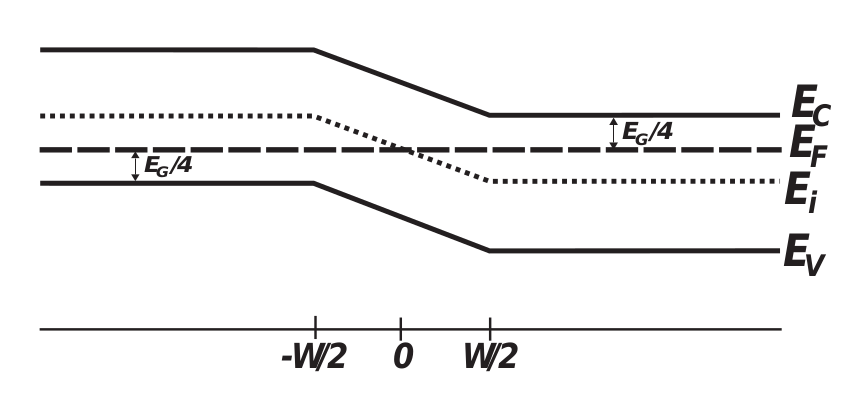
\includegraphics[width=0.7\linewidth]{Ejercicios/Ch_02/02_Ejercicio_15.png}		
\end{center}

\begin{itemize}
	\item[(a)] Si el semiconductor de Si se mantiene a temperatura ambiente, determinar la resistividad del semiconductor para la región \(x > W/2\). Para los electrones en la región \(x > W/2\) que intentan moverse a la región \(x < -W/2\) sin modificar su energía total, ¿cuál es la mínima energía cinética que deben tener?
	\item[(b)] Calcular y representar gráficamente el potencial electrostático y el campo eléctrico en función de \(x\). Explicar si el semiconductor está en equilibrio termodinámico.
	\item[(c)] Responder las siguientes preguntas:
		  \begin{itemize}
			  \item ¿Cuál es la densidad de corriente de electrones (\(J_n\)) y de huecos (\(J_p\)) en \(x = 0\)?
			  \item ¿Existe corriente de arrastre de electrones en \(x = 0\)? Si así fuera, ¿cuál es la dirección del flujo de corriente de arrastre?
			  \item ¿Existe corriente de difusión de electrones en \(x = 0\)? En tal caso, ¿cuál es la dirección del flujo de corriente de difusión?
			\end{itemize}
  \end{itemize}
\end{Enunciado}




\begin{enumerate}[label=\alph*)]
	\item La resisitividad, como hemos visto a lo largo de todos los ejericcios, viene dada por:
	\begin{equation}
		\rho = \frac{1}{q(\mu_n n + \mu_p p)}
	\end{equation}
	Por lo que solo tenemos que calcular $n$ y $p$ para $\mu_n$ y $\mu_p$ dados (valores que tendremos que coger de otro ejercicio). Así pues, obtenemos $n$ y $p$ a partir de las ecuaciones:

	\begin{equation}
		n = n_i e^{(E_F-E_i)/kT} \qquad p = n_i e^{(E_i-E_F)/kT}
	\end{equation}
	Donde conocemos $N_C$ y $N_V$ a 300K (temperatura ambiente) y la diferencia de $E_c-E_F=E_g/4$ y $E_F-E_v=3E_g/4$ en $x>W/2$ (véase diagrama de bandas). Así pues conocemos los valores:

	\begin{equation}
		n= 7.91\times 10^{14} \ \cm^{-3} \tquad p = 4.5\times 10^{14} \ \cm^{-3}
	\end{equation}
	Usando las siguientes movilidades (calculadas con las ecuacioens de portadores mayoritarios/minoritarios previas):
	
	\begin{equation}
		\mu_n = 1290 \ \cm^2 /  \text{V s} \tquad \mu_p = 499 \ \cm^2 /  \text{V s}
	\end{equation}
	tal que la resistividad en $W/2<x$:

	\begin{equation}
		\rho = 5.02 \ \Omega \cm
	\end{equation}
	\textcolor{red}{Da 7.73. En gneral hacen aproximaciones ignorando uno de los portadores.} Ahora solo queda calcualar la energía cinética mínima $T_{\min}$ que deben tener. Como podemos ver la energía de la banda de conducción aumenta de la región $x>W/2$ a la región $x<W/2$. Así pues:

	\begin{equation}
		T_{\min} = E_c(-W/2) - E_c(W/2) = E_g/2 = 0.506 \	 \eV
	\end{equation}
	\item Como sabemos el campo eléctrico viene dado por:
	\begin{equation} 
		\Ecal = \frac{1}{q} \derivadas{E_i}{x}
	\end{equation}
	y el potencial $V(x)=-E_i(x)+V_0$ donde $V_0$ es una constate arbitraria que nos ayuda a redefinir el cero del potencial. Como para calcular la derivada (y $V_0$ siempre nos permite redefinir el cero de $V$) solo necesitamos conocer la \textit{dependencia de $E_i$ con la posición}, podemos escribir 

	\begin{equation}
		E_i = E_{i0} - \frac{E_g}{2} \frac{x}{W}
	\end{equation}
	siendo $E_{i0}$ una constante irrelevante que contiene información de la energía respecto al cero $E_F=0$ eV. Así pues:

	\begin{equation}
		\Ecal = - \frac{1}{q} \frac{E_g}{2W}
	\end{equation}
	Así pues:

	\begin{equation}
		V=V_0 + \frac{E_g}{q} \frac{x}{2W} 
	\end{equation}
	Para ver si está en equilibrio termodinámico tenemos que ver si $J_n=J_p=0$. Veamos que $J_n=0$ implica que:

	\begin{equation}
		J_n = J_n |_{\text{difusion}} +J_n |_{\text{arrastre}} = q\mu_n n \Encal + qD_n\derivadas{n}{x} = 0
	\end{equation}
	De tal modo que, si estamos en equilibrio se tiene que verificar que
	\begin{equation}
		\Ecal_n = \frac{D_n}{\mu_n} \frac{1}{n} \derivadas{n}{x} = 
		\frac{kT}{q} \frac{1}{n} \derivadas{n}{x}
	\end{equation} 
	donde hemos aplicado las reglas de Einstein (válido para el equlibrio y fuera del equlibrio). Ahora solo tenemos que evaluar $n(x)$ y su derivada. Es sencillo de ver que la única dependencia mostrada en el diagrama de bandas:

	\begin{equation}
		n = \left\lbrace
		\begin{array}{ll}
			N_c e^{-\frac{1}{kT}\frac{3E_g}{4}}	& \text{si} \ x<-W/2 \\
			N_c e^{-\frac{1}{kT}\frac{E_g}{4} \parentesis{\frac{-x+W}{W/2}}}	& \text{si} \ -W/2<x<W/2 \\
			N_c e^{-\frac{1}{kT}\frac{E_g}{4}} & \text{si} \ W/2<x
		\end{array} \right.
	\end{equation}
	De lo cual deducimos que la derivada es:

	\begin{equation}
		\derivadas{n}{x} = \left\lbrace
		\begin{array}{ll}
			0	& \text{si} \ x<-W/2 \\
			\frac{1}{kT}\frac{E_g}{4}\frac{2}{W}N_c e^{-\frac{1}{kT}\frac{E_g}{4} \parentesis{\frac{-x+W}{W/2}}}	& \text{si} \ -W/2<x<W/2 \\
			0 & \text{si} \ W/2<x
		\end{array} \right.
	\end{equation}
	Consecuentemente el campo eléctrico:

	\begin{equation}
		\Ecal_n = - \frac{1}{q} \frac{E_g}{2W}   \qquad \text{si} \ - W/2<x<W/2
	\end{equation}  
	Que como podemos ver es la misma expresión. Para los portadores huecos se puede llegar a lo mismo siguiendo los mismos pasos (la única diferencia es que aparecen dos signos menos que se cancelan). Veamos como quedan las gráficas:

	\begin{center}
		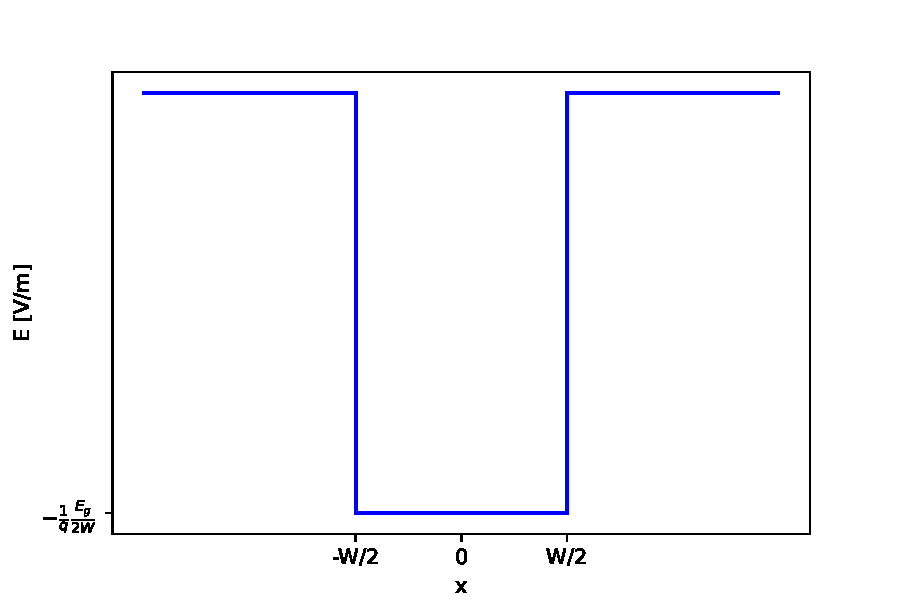
\includegraphics[width=0.7\linewidth]{Ejercicios/Ch_02/02_Ejercicio_15_E(x).pdf}
	\end{center}
	\begin{center}
		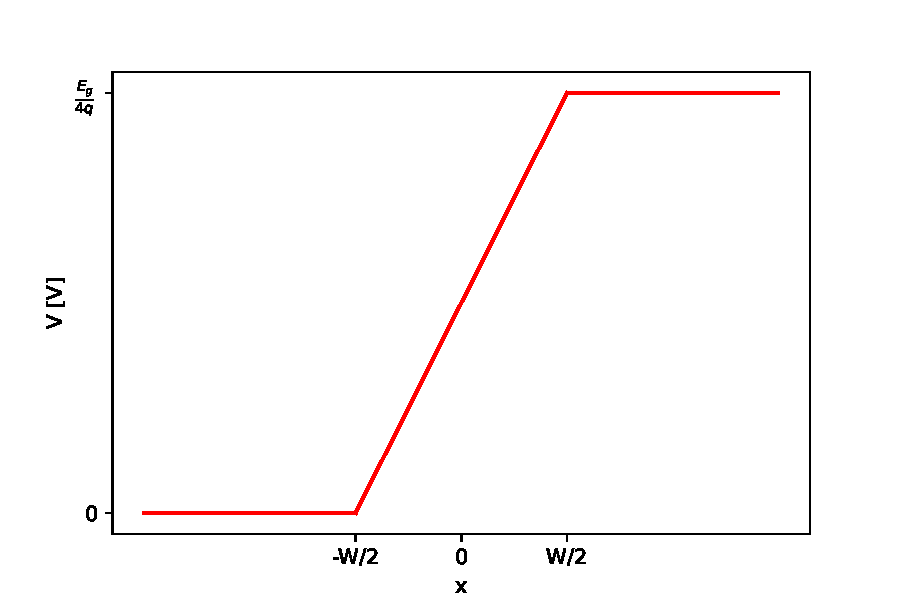
\includegraphics[width=0.7\linewidth]{Ejercicios/Ch_02/02_Ejercicio_15_V(x).pdf}
	\end{center}

	\item Respondemos a cada una de las preguntas:
	\begin{itemize}
		\item La densidad de corriente de electrones y de huecos en $x=0$ es cero, como hemos visto en el apartado anterior. De otra manera no estaríamos en el equilibrio termodinámico.
		\item Corriente de arrastre hay, ya que el campo eléctrico no es nulo (en $x=0$). Así pues: 
		\begin{equation}
			\Jn_n |_{\text{arrastre}} = q \mu_n n \Encal =  - \mu_n \frac{E_g}{2W} N_c  e^{-\frac{1}{kT}\frac{E_g}{2}}  \hnx 
		\end{equation}
		Lógicamente la corriente de arrastre tiene que tener la misma dirección que la corriente eléctrica, ya que aún que la velocidad del electrón tendrá la dirección contraria al campo eléctrico y la corriente de carga tendrá la dirección contraria a la velocidad del electrón. 
		\item Corriente de difusión hay, y en virtud de que $\Jn_n|_{\text{arrastre}}=- \Jn_n|_{\text{difusion}}$, tenemos que
		\begin{equation}
			\Jn_n |_{\text{arrastre}} = - q \mu_n n \Encal =  \mu_n \frac{E_g}{2W} N_c  e^{-\frac{1}{kT}\frac{E_g}{2}}  \hnx 
		\end{equation}
	\end{itemize}
\end{enumerate}


\begin{Enunciado}
\subsection*{Ejercicio 8}

Interpretación de un diagrama de bandas de energía para un semiconductor de silicio tomando $L=1$ micra:
\begin{center}
	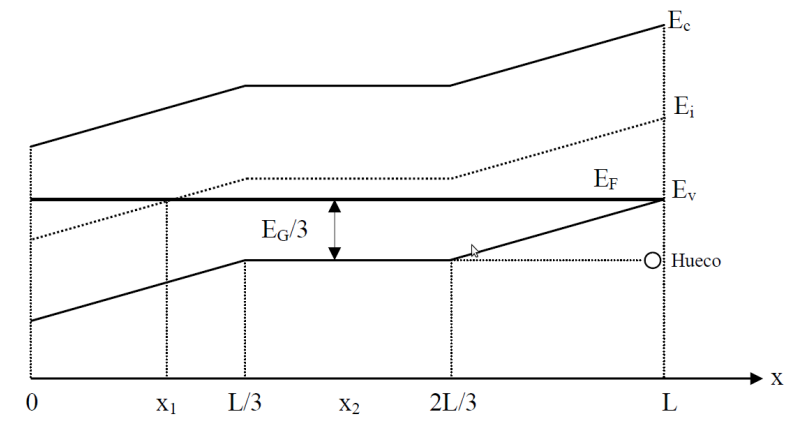
\includegraphics[width=0.7\linewidth]{Ejercicios/Ch_02/02_Ejercicio_16.png}		
\end{center}
\begin{itemize}
	\item[(a)] Calcula y representa graficamente el potencial electrostático y el campo eléctrico en el interior del semiconductor. Determina si el sistema esta o no en equilibrio termodinámico.
	\item[(b)] Calcula si el semiconductor es degenrado en alguna zona. En $x=x_2$, ¿a qué es igual $p$?
	\item[(c)] Captura la densidad de corriente de electrones $J_n$ y la densidad de corriente de arrastre de huecos $J_p^a$ que fluye en $x=x_1$. Determina cuanto vale la energía cinética del hueco que aparece en el diagrama en la posición $x=L$. 
\end{itemize}

\end{Enunciado}




\begin{enumerate}[label=\alph*)]
	\item Queremos calcular el potencial electrostático y el campo eléctrico en el interior del semiconductor. Usamos la misma relación que en el ejercicio anterior:
	\begin{equation}
		\Ecal = \frac{1}{q} \derivadas{E_i}{x}
	\end{equation}
	Veamos que la energía varía como:
	\begin{equation}
		E_i(x) = \left\lbrace \begin{array}{ll}
			\frac{E_{i0}}{L/3-x_1} (x-x_1) \quad & \ \text{si} \ x<L/3 \\
			E_{i0} \quad & \ \text{si} \ L/3<x2L/3 \\
			E_{i0+\frac{E_{i0}}{L/3-x_1} (x-2L/3)} \quad & \ \text{si} \ 2L/3<x
		\end{array} \right.
	\end{equation}
	Recordamos que en $L/3$ tenemos que $E_v=-E_g/3$, y por tanto $E_c=2E_g/3$, tal que $E_{i0}=E_g/6+(3kT/4)\cdot \log(m_n^*/m_p^*)=0.179 \ \eV$, donde hemos redefinido $E_F=0$. Por lo que igual que antes tenemos que el campo eléctrico viene dado por regiones:
	\begin{equation}
		\Ecal(x) = \left\lbrace \begin{array}{ll}
			\frac{E_{i0}}{L/3-x_1} \quad & \ \text{si} \ x<L/3\\
			0 \quad & \ \text{si} \ L/3<x2L/3 \\
			\frac{E_{i0}}{L/3-x_1} \quad & \ \text{si} \ 2L/3<x
		\end{array} \right.
	\end{equation}
	y por tanto:

	\begin{equation}
		V(x) = \left\lbrace \begin{array}{ll}
			V_0 -\frac{E_{i0}}{L/3-x_1} (x-L/3) \quad & \ \text{si} \ x<L/3 \\
			V_0 \quad & \ \text{si} \ L/3<x2L/3 \\
			V_0 -\frac{E_{i0}}{L/3-x_1} (x-2L/3) \quad & \ \text{si} \ 2L/3<x
		\end{array} \right.
	\end{equation}
	Ahora solo tendríamos que hacer el esquema:

	\begin{center}
		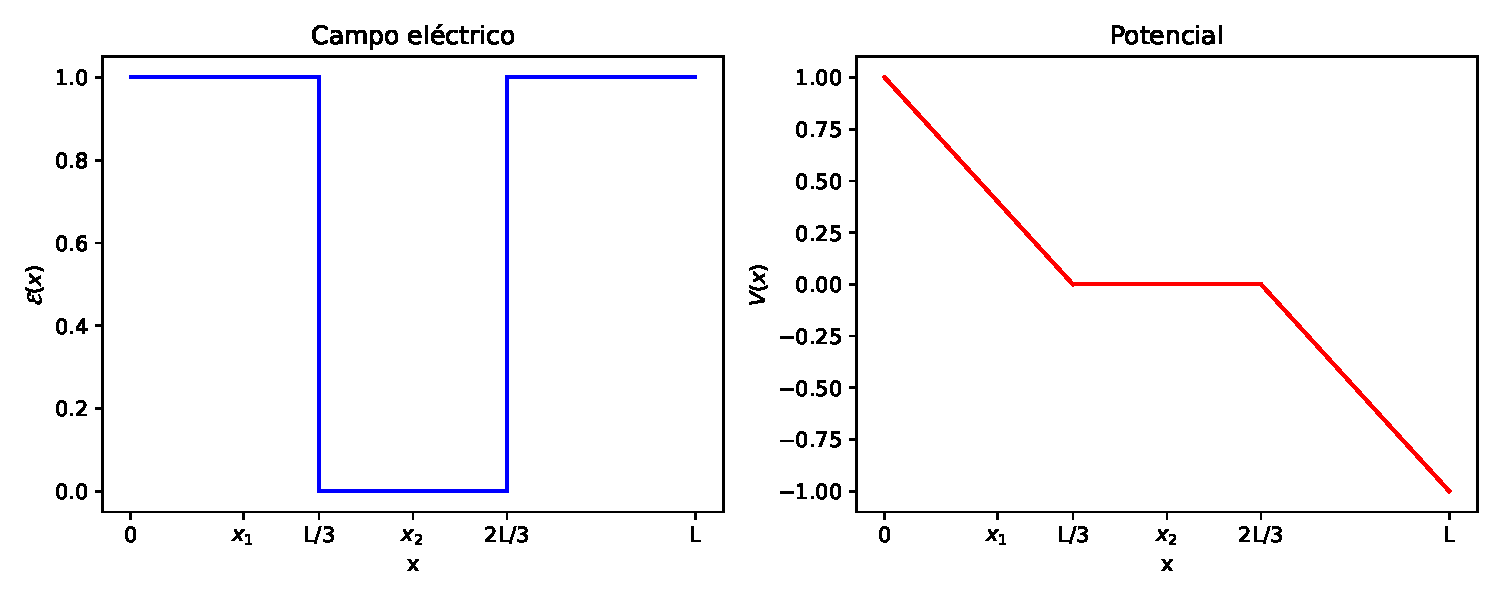
\includegraphics[width=\linewidth]{Ejercicios/Ch_02/02_Ejercicio_16.pdf}
	\end{center}
		
	Para determinar que está en equilibrio basta ver que $\Jn_T=0$ y que $T=\cte$, lo cual es cierto. Para ver que $\Jn=0$ debemos seguir el mismo procedimiento que antes.
	\item  Evidentemente es degenerado en $x=L$, ya que $E_F=E_v$. En $x_2$ tenemos que: 
	\begin{equation}
		p = N_V e^{\frac{E_F-E_v}{kT}} = N_V e^{\frac{E_g}{3kT}} = n_i e^{\frac{E_F-E_i}{kT}}
	\end{equation}
	tal que en $x_2$ tenemos que $E_i=E_{i0}=0.179 \ \eV$. Los datos:

	\begin{equation}
		p = 1.22 \times 10^{13} \ \cm^{-3}
	\end{equation}
	\item Nos piden la densidad de corriente de electrones $J_n$ y la densidad de corriente de huecos en $x=x_1$. Es exactamente igual que en el anterior ejercicio:
	\begin{equation}
		\Jn|_{\text{{arrastre}}} = q \mu_n n \Encal = 0
	\end{equation}
	ya que en $x_1$ no hay corriente. La energía cinética del hueco $T$ viene dada por la diferencia entre $E_v=0$ (en $x=L$) y $-E_g/3$. Así pues:

	\begin{equation}
		T = - \frac{-E_g}{3}
	\end{equation}
	por suponer, ya que no tenemos ningún tipo de motivación para suponer que es así. 

\end{enumerate}








